\section{Evaluación}\label{sec:eval}

Como parte fundamental de la creación de un SRI se tiene el proceso de
evaluación, donde se determinará la eficacia del mismo.

Para la evaluación del modelo propuesto se cuenta, como procedimiento estándar,
con varias colecciones de pruebas, las cuales contienen lo siguiente:

\begin{enumerate}
    \item Una colección de documentos.
    \item Un conjunto de pruebas a realizar sobre la colección, llamadas
    consultas (\emph{queries}).
    \item Un conjunto de juicios de relevancia, una evaluación mayormente
    binaria sobre la relevancia de las consultas sobre los documentos (en
    algunas de las colecciones utilizadas el espectro de evaluación no es tan
    binario) 
\end{enumerate}

Sobre la estructura de las colecciones utilizadas y descritas con anterioridad,
trabaja el modelo, se realizan comparaciones y cálaculo de métricas que
caracterizan la efectividad del mismo.

\subsection{Métricas empleadas}\label{sec:metrics}

Para realizar un análisis de la efectividad de cada modelo se emplearon 
dversas métricas. Primero, se define como:

\begin{itemize}
	\item RR: Documentos relevantes recuperados.
	\item RI: Documentos irelevantes recuperados.
	\item NR: Documentos relevantes no recuperados.
	\item NI: Documentos irelevantes no recuperados.
	\item P: Precisión.
	\item R: Recobrado.
\end{itemize}

Luego, las métricas usadas son:

\begin{itemize}
\item Precisión:
    $$P = \dfrac{|RR|}{|RR \cup RI|}$$
    Denota la proporción de los documentos relevantes recuperados sobre
	el total de documentos recuperados.\\
\item Recobrado (Recall):
    $$R = \dfrac{|RR|}{|RR \cup NR|}$$
	Denota la proporción de los documentos relevantes recuperados sobre
	el total de documentos relevantes.\\
\item Medida $F_1$:
    $$F_1 = \dfrac{2PR}{P+R} = \dfrac{2}{\frac{1}{P} + \frac{1}{R}}$$
    Medida que armoniza entre Precisión y Recobrado.\\
\item Fallout:
	$$Fallout = \dfrac{|RI|}{|RI\cup NI|}$$
     Denota la cantidad de documentos irrelevantes recuperados sobre el total de
	 documentos irrelevantes.
\end{itemize}

\subsection{Proceso de evaluación}\label{sec:evaluation}

Para describir el proceso de evaluación primero es necesario definir el concepto
de \emph{tope}. Este concepto se define como: los primeros $k$ documentos
resultantes de una consulta.

En el análisis de un modelo se calculan las métricas antes mencionadas, por
cada consulta, para diferentes topes. De estas métricas se extraen valores
estadísticos relevantes como: la media, la desviación estándar, el máximo y
el mínimo, por cada uno de los topes establecido ($2, 4, 6, ..., 50$). Se
analiza además, el comportamiento del promedio de las relevancias.

De esta forma para cada modelo se puede analizar el comportamiento de las métricas
estudiadas a medida que aumentamos la cantidad de documentos recuperados. En las
figuras \ref{fig:cran-eval} y \ref{fig:med-eval} se muestran los resultados
para el modelo de Cran y el modelo de Medline respectivamente. Como se puede
observar, el modelo de Medline, presenta una mayor efectividad.

Se puede apreciar en ambos resultados como el la precisión va disminuyendo y 
el recobrado va aumentando a medida que aumentan la cantidad de documentos
recuperados.

Es notable además que ambos modelos presentan un comportamiento similar con
respecto al promedio de relevancia obtenido en cada tope. Esto muestra que
este valor por si solo no es una métrica útil. No obstante, es interesante
analizar su comportamiento en función de la cantidad de documentos recuperados.

\begin{figure}[htb]%
	\begin{center}
		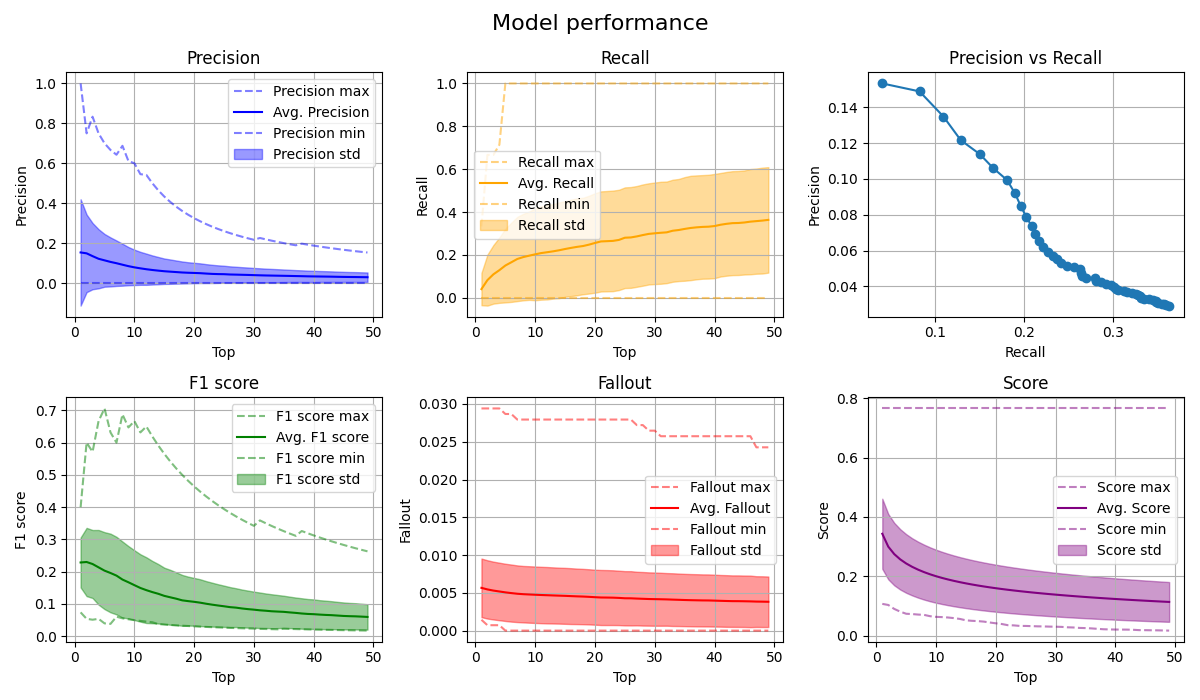
\includegraphics[width=1.0\textwidth]{./cran_eval.png}
	\end{center}
	\caption{Evaluación del modelo de la base de datos de \emph{cran}}
	\label{fig:cran-eval}
\end{figure}


\begin{figure}[htb]%
	\begin{center}
		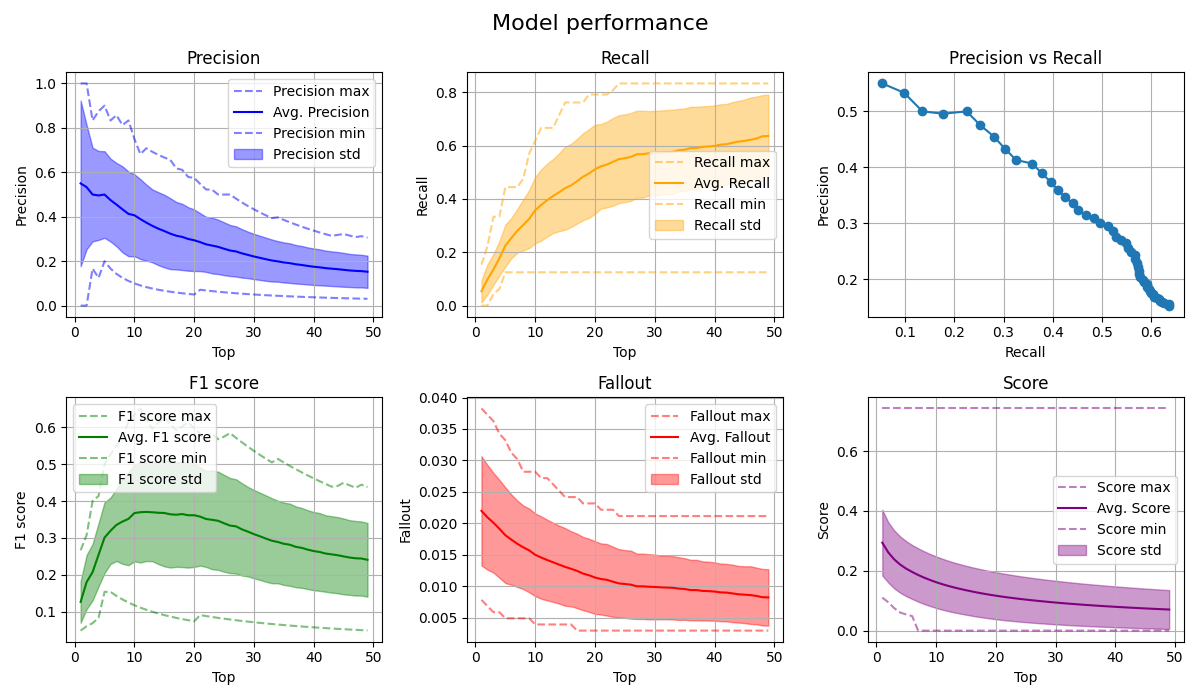
\includegraphics[width=1.0\textwidth]{./med_eval.png}
	\end{center}
	\caption{Evaluación del modelo de la base de datos de \emph{med}}
	\label{fig:med-eval}
\end{figure}

Además de la evaluación de un modelo determinando, la aplicación desarrollada
permite mostrar una comparación entre modelos creados con diferentes
parámetros para una misma base de datos. En la figura \ref{fig:cran-comp} se muestra
la comparación entre dos modelos de la base de datos de \emph{cran}. Uno de ellos
(líneas discontinuas) fue construído con una tokenización simple (split), sin
lemtizar, sin stemming, sin quitar las palabras comunes. El otro, por otra parte,
fue construído con utilizando el método de tokenización de \emph{nltk}, con
stemming, lematización, quitando las palabras comunes.

\begin{figure}[htb]%
	\begin{center}
		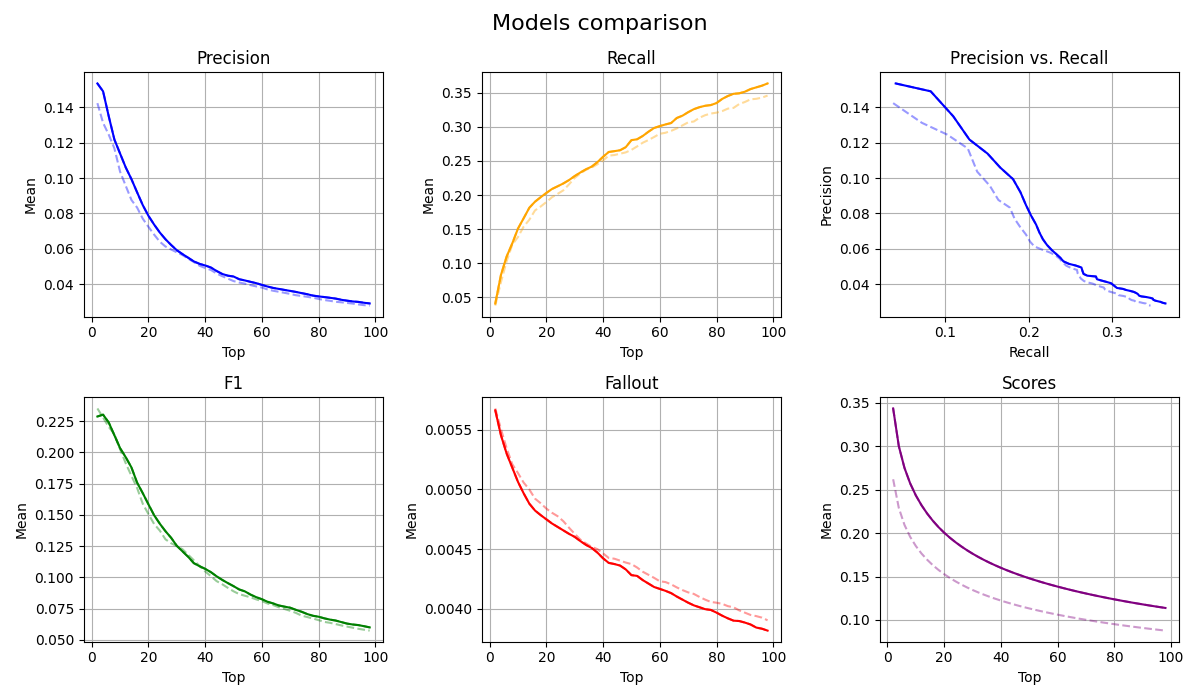
\includegraphics[width=1.0\textwidth]{./cran_comp.png}
	\end{center}
	\caption{Comparación de diferentes modelos para la base de datos de \emph{cran}}
	\label{fig:cran-comp}
\end{figure}

Como se puede apreciar, con el nuevo modelo se obtuvo una pequeña mejora en la
precisión y el recobrado. Se muestra también cómo el promedio de fallos disminuyó.
